\documentclass[12pt]{beamer}
\usepackage{../Estilos/BeamerMAF}
\usepackage{../Estilos/ColoresLatex}
\usepackage[absolute, overlay]{textpos}

\usetheme{Copenhagen}
\usecolortheme{wolverine}
%\useoutertheme{default}
\setbeamercovered{invisible}
% or whatever (possibly just delete it)
\setbeamertemplate{section in toc}[sections numbered]
\setbeamertemplate{subsection in toc}[subsections numbered]
\setbeamertemplate{subsection in toc}{\leavevmode\leftskip=3.2em\rlap{\hskip-2em\inserttocsectionnumber.\inserttocsubsectionnumber}\inserttocsubsection\par}
% \setbeamercolor{section in toc}{fg=blue}
% \setbeamercolor{subsection in toc}{fg=blue}
% \setbeamercolor{frametitle}{fg=blue}
\setbeamertemplate{caption}[numbered]

\setbeamertemplate{footline}
\beamertemplatenavigationsymbolsempty
\setbeamertemplate{headline}{}


\makeatletter
% \setbeamercolor{section in foot}{bg=gray!30, fg=black!90!orange}
% \setbeamercolor{subsection in foot}{bg=blue!30}
% \setbeamercolor{date in foot}{bg=black}
\setbeamertemplate{footline}
{
  \leavevmode%
  \hbox{%
  \begin{beamercolorbox}[wd=.333333\paperwidth,ht=2.25ex,dp=1ex,center]{section in foot}%
    \usebeamerfont{section in foot} \insertsection
  \end{beamercolorbox}%
  \begin{beamercolorbox}[wd=.333333\paperwidth,ht=2.25ex,dp=1ex,center]{subsection in foot}%
    \usebeamerfont{subsection in foot}  \insertsubsection
  \end{beamercolorbox}%
  \begin{beamercolorbox}[wd=.333333\paperwidth,ht=2.25ex,dp=1ex,right]{date in head/foot}%
    \usebeamerfont{date in head/foot} \insertshortdate{} \hspace*{2em}
    \insertframenumber{} / \inserttotalframenumber \hspace*{2ex} 
  \end{beamercolorbox}}%
  \vskip0pt%
}
\makeatother

\makeatletter
\patchcmd{\beamer@sectionintoc}{\vskip1.5em}{\vskip0.8em}{}{}
\makeatother

% %\newlength{\depthofsumsign}
% \setlength{\depthofsumsign}{\depthof{$\sum$}}
% \newcommand{\nsum}[1][1.4]{% only for \displaystyle
%     \mathop{%
%         \raisebox
%             {-#1\depthofsumsign+1\depthofsumsign}
%             {\scalebox
%                 {#1}
%                 {$\displaystyle\sum$}%
%             }
%     }
% }
% \def\scaleint#1{\vcenter{\hbox{\scaleto[3ex]{\displaystyle\int}{#1}}}}
% \def\scaleoint#1{\vcenter{\hbox{\scaleto[3ex]{\displaystyle\oint}{#1}}}}
% \def\bs{\mkern-12mu}


\resetcounteronoverlays{saveenumi}

\AtBeginDocument{\RenewCommandCopy\qty\SI}
\ExplSyntaxOn
\msg_redirect_name:nnn { siunitx } { physics-pkg } { none }
\ExplSyntaxOff

\date{}

\title{\large{Funciones de Chebyshev}}
\subtitle{Tema 4 - Funciones Especiales}
\author{M. en C. Gustavo Contreras Mayén}

\resetcounteronoverlays{saveenumi}

\begin{document}
\maketitle
\fontsize{14}{14}\selectfont
\spanishdecimal{.}

\section*{Contenido}
\frame[allowframebreaks]{\frametitle{Contenido} \tableofcontents[currentsection, hideallsubsections]}

%Referencia Riley 18.4 Chebyshev functions
\section{Funciones de Chebyshev}
\frame[allowframebreaks]{\frametitle{Temas a revisar} \tableofcontents[currentsection, hideothersubsections]}
\subsection{Ec. Diferencial}

\begin{frame}
\frametitle{Ec. Diferencial de partida}
La ecuación diferencial de Chebyshev tiene la forma:
\pause
\begin{align}
(1 - x^{2}) \, \sderivada{y} - x \, \pderivada{y} + \nu^{2} \, y
 = 0
 \label{eq:ecuacion_18_054}
\end{align}
y tiene tres puntos singulares regulares, en $x = -1, 1, \infty$.
\end{frame}

% Al comparar la ecuación con:
% \begin{align*}
% (1 - x^{2}) \, \sderivada{y} - x \, \pderivada{y} + \ell (\ell + 1) \, y = 0
% \end{align*}
%vemos que la ecuación de Chebyshev es muy similar en forma a la ecuación de Legendre. A pesar de esta similitud,
\begin{frame}
\frametitle{Frecuencia de la ED}
La ecuación (\ref{eq:ecuacion_18_054}) no se presenta con mucha frecuencia en problemas físicos, aunque \textocolor{byzantium}{sus soluciones son de considerable importancia en el análisis numérico}.
\end{frame}
\begin{frame}
\frametitle{Estudiando la ED}
El parámetro $\nu$ es un número real dado, pero en casi todas las aplicaciones prácticas toma un valor entero.
\\
\bigskip
\pause
De aquí en adelante asumimos que $\nu = n$, donde $n$ es un número entero no negativo.
\end{frame}
\begin{frame}
\frametitle{Cambio de argumento}
%Como fue el caso de la ecuación de Legendre, en 
El uso normal la variable $x$ es el coseno de un ángulo, por lo que $-1 \leq x \leq 1$.
\\
\bigskip
\pause
Cualquier solución de la ec. (\ref{eq:ecuacion_18_054}) se llama \textocolor{cobalt}{función de Chebyshev}.
\end{frame}
\begin{frame}
\frametitle{Puntos ordinarios en la ED}
El punto $x = 0$ es un punto ordinario de la ec. (\ref{eq:ecuacion_18_054}), por lo que esperamos encontrar
dos soluciones linealmente independientes de la forma:
\pause
\begin{align*}
y = \nsum_{m=0}^{\infty} a_{m} \, x^{m}
\end{align*}
\end{frame}
\begin{frame}
\frametitle{Estrategia distinta}
Se podrían encontrar las relaciones de recurrencia para los coeficientes $a_{m}$.% de una manera similar a la utilizada para la ecuación de Legendre. Para la ecuación de Chebyshev, sin embargo, 
\\
\bigskip
\pause
Es más fácil y esclarecedor adoptar un enfoque diferente.
\end{frame}
\begin{frame}
\frametitle{Cambio de argumento}
En particular, notamos que, al hacer la sustitución $x = \cos \theta$, y en consecuencia:
\pause
\begin{align*}
\dv{x} = \left( \dfrac{-1}{\sin \theta} \right) \, \dv{\theta}
\end{align*}
\end{frame}
\begin{frame}
\frametitle{Cambio de argumento}
La ecuación de Chebyshev se convierte en (con $\nu = n$):
\pause
\begin{align*}
\dv[2]{y}{\theta} + n^{2} \, y = 0
\end{align*}
que corresponde a la ecuación del oscilador armónico simple, con solución $\cos n \theta$ y $\sin n \theta$. 
\end{frame}
\begin{frame}
\frametitle{Soluciones a la ED}
Las correspondientes soluciones linealmente independientes de la ecuación de Chebyshev están dadas por:
\pause
\begin{align}
\begin{aligned}
T_{n} (x) &= \cos (n \, \cos^{-1} x) \\[0.5em]
V_{n} (x) &= \sin (n \, \cos^{-1} x)
\end{aligned}
\label{eq:ecuacion_18_055}
\end{align}
\end{frame}
\begin{frame}
\frametitle{Soluciones con polinomios}
Es sencillo demostrar que los $T_{n} (x)$ son polinomios de orden $n$, mientras que $V_{n} (x)$ no son polinomios.
\end{frame}

\subsection{Forma explícita de \texorpdfstring{$T_{n}(x)$}{T(n)(x)} y \texorpdfstring{$V_{n}(x)$}{Vn(x)}.}

\begin{frame}
\frametitle{Manejando el argumento}
Escribiendo $x = \cos \theta$, conviene primero formar la superposición compleja:
\pause
\begin{eqnarray*}
\begin{aligned}
T_{n} (x) + i \, V_{n} (x) &= \cos n \theta + i \, \sin n \theta = \\[0.5em] \pause
&= (\cos \theta + i \, \sin \theta)^{n} = \\[0.5em] \pause
&= \left( x + i \, \sqrt{1- x^{2}} \right)^{n} \hspace{1cm} \mbox{para  } \abs{x} \leq 1
\end{aligned}
\end{eqnarray*}
\end{frame}
\begin{frame}
\frametitle{Desarrollando el binomio}
Entonces, al expandir la última expresión con el teorema binomial, obtenemos:
\pause
\begin{align}
\begin{aligned}
T_{n} (x) &= x^{n} - \binom{n}{2} \, x^{n-2} \, (1 - x^{2}) + \\[1em]
&+ \binom{n}{4} \, x^{n-4} \, (1 - x^{2})^{2} - \ldots
\end{aligned}
\label{eq:ecuacion_18_056}
\end{align}
\end{frame}
\begin{frame}
\frametitle{Desarrollando el binomio}
\begin{align}
\begin{aligned}[b]
V_{n} (x) &= \sqrt{1 {-} x^{2}} \, \bigg[ \binom{n}{1} \, x^{n-1} {-} \binom{n}{3} \, x^{n-3} \, (1 {-} x^{2}) + \\[0.5em]
&+ \binom{n}{5} \, x^{n-5} \, (1 {-} x^{2})^{2} + \ldots \bigg]
\end{aligned}
\label{eq:ecuacion_18_057}
\end{align}
De esta manera vemos que $T_{n} (x)$ es un polinomio de orden $n$, pero $V_{n} (x)$ no es un polinomio.
\end{frame}

\subsection{Funciones adicionales}

\begin{frame}
\frametitle{Nuevas funciones}
Es conveniente definir las funciones adicionales:
\pause
\begin{align}
\begin{aligned}
W_{n} (x) &= (1 - x^{2})^{-1/2} \, T_{n+1} (x) \\[0.5em]
U_{n} (x) &= (1 - x^{2})^{-1/2} \, V_{n+1} (x)
\end{aligned}
\label{eq:ecuacion_18_058}
\end{align}
\end{frame}
\begin{frame}
\frametitle{Funciones que son polinomios}
De las ecs. (\ref{eq:ecuacion_18_056}) y (\ref{eq:ecuacion_18_057}), vemos de inmediato que $U_{n}(x)$ es un \textocolor{lava}{polinomio de orden n}, mientras que $W_{n}(x)$ no lo es.
\end{frame}
\begin{frame}
\frametitle{Polinomios de Chebyshev}
En la práctica, es habitual trabajar íntegramente en términos de los $T_{n} (x)$ y $U_{n} (x)$, que se conocen, respectivamente, como los \textocolor{ao}{polinomios de Chebyshev de primer y segundo tipo}.
\end{frame}
\begin{frame}
\frametitle{Solución general a la ED}
En particular, observamos que la solución general de la ecuación de Chebyshev se puede escribir en términos de estos polinomios como:
\pause
\begin{align*}
y (x) = \begin{cases}
c_{1} T_{n} (x) {+} c_{2} \sqrt{1 {-} x^{2}} U_{n-1} (x) & \!\!\!\! \mbox{para } n {=} 1, 2, \ldots \\[0.5em]
c_{1} + c_{2} \, \sin^{-1} x & \mbox{para  } n = 0
\end{cases}
\end{align*}
\end{frame}
\begin{frame}
\frametitle{Solución particular a la ED}
La solución con $n = 0$ se puede escribir como:
\pause
\begin{align*}
d_{1} + c_{2} \, \cos^{-1} x \hspace{1.5cm} \mbox{con  } d_{1} = c_{1} + \dfrac{1}{2} \, \pi \, c_{2}
\end{align*}
\end{frame}
\begin{frame}
\frametitle{Primeros polinomios}
Los primeros polinomios de Chebyshev de primer tipo se pueden construir fácilmente y están dado por:
\pause
\begin{table}[H]
\centering
\fontsize{14}{14}\selectfont
\begin{tabular}{p{4.45cm} p{5.5cm}}
$T_{0} (x) {=} 1$ & $T_{1} (x) {=} x$ \\[0.25em]
$T_{2} (x) {=} 2 \, x^{2} {-} 1$ & $T_{3} (x) {=} 4 \, x^{3} {-} 3 \, x$ \\[0.25em]
$T_{4} (x) {=} 8 \, x^{4} {-} 8 \, x^{2} {+} 1$ & $T_{5} (x) {=} 16 \, x^{5} {-} 20 \, x^{3} {+} 5 \, x$ \\
\vdots & \vdots
\end{tabular}
\end{table}
\end{frame}
\begin{frame}
\frametitle{Primeros polinomios}
En la figura (\ref{fig:figura_plot_chebychev_01}) se presenta la gráfica de los primeros polinomios de Chebyshev de primera clase.
\end{frame}
\begin{frame}
\frametitle{Primeros polinomios}
\begin{figure}[H]
    \centering
    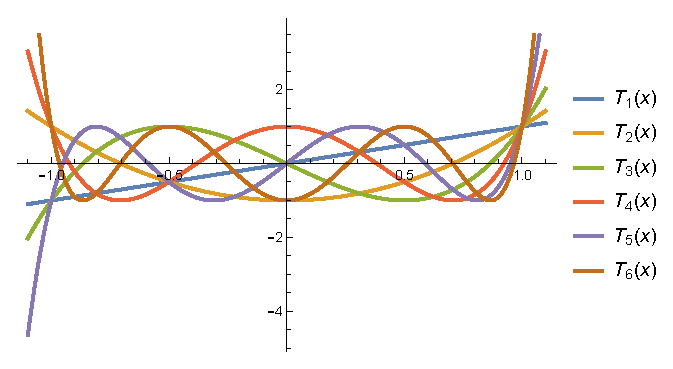
\includegraphics[scale=0.85]{Imagenes/Plot_Polinomios_Chebychev_01.eps}
    \caption{Primeros polinomios de Chebyshev de primera clase.}
    \label{fig:figura_plot_chebychev_01}
\end{figure}
\end{frame}
\begin{frame}
\frametitle{Paridad de los $T_{n} (x)$}
En general, los polinomios de Chebyshev $T_{n} (x)$ satisfacen:
\pause
\begin{align*}
T_{n} (-x) = (-1)^{n} \, T_{n} (x)
\end{align*}
que se puede deducir fácilmente a partir de la ec. (\ref{eq:ecuacion_18_056}).
\end{frame}
\begin{frame}
    \frametitle{Primeras relaciones}
También es fácil deducir los siguientes valores especiales:
\pause
\begin{align*}
T_{n} (1) &= 1 \\[0.5em]
T_{n} (-1) &= (-1)^{n} \\[0.5em]
T_{2n} (0) &= (-1)^{n} \\[0.5em]
T_{2n+1} (0) &= 0
\end{align*}
\end{frame}
\begin{frame}
\frametitle{Polinomios de segunda clase}
Los primeros polinomios de Chebyshev de segunda clase se pueden obtener fácilmente, se presentan a continuación los primeros:
\end{frame}
\begin{frame}
\frametitle{Polinomios de segunda clase}
\begin{table}[H]
\centering
\fontsize{14}{14}\selectfont
\begin{tabular}{p{4.8cm} p{5cm}}
$U_{0} (x) {=} 1$ & $U_{1} (x) {=} 2 \, x$ \\[0.5em]
$U_{2} (x) {=} 4 \, x^{2} {-} 1$ & $U_{3} (x) {=} 8 \, x^{3} {-} 4 \, x$ \\[0.5em]
$U_{4} (x) {=} 16 \, x^{4} {-} 12 \, x^{2} {+} 1$ & $U_{5} (x) {=} 32 \, x^{5} {-} 32 \, x^{3} {+} 6 \, x$ \\
\vdots & \vdots
\end{tabular}
\end{table}
\end{frame}
\begin{frame}
\frametitle{Gráfica de lo polinomios de segunda clase}
Las funciones que representan a los polinomios de Chebyshev de segunda clase se presentan en la figura (\ref{fig:figura_plot_chebychev_02}):
\end{frame}
\begin{frame}
\frametitle{Gráfica de lo polinomios de segunda clase}
\begin{figure}[H]
    \centering
    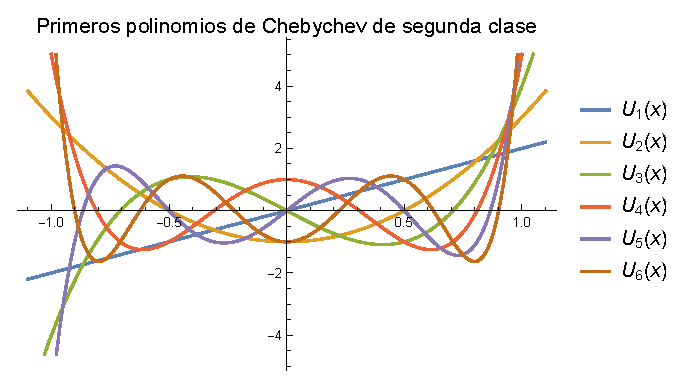
\includegraphics[scale=0.95]{Imagenes/Plot_Polinomios_Chebychev_02.eps}
    \caption{Primeros polinomios de Chebyshev de segunda clase.}
    \label{fig:figura_plot_chebychev_02}
\end{figure}
\end{frame}
\begin{frame}
\frametitle{Propiedad de los $U_{n} (x)$}
Los polinomios de Chebyshev $U_{n} (x)$ también satisfacen la propiedad:
\pause
\begin{align*}
U_{n} (-x) = (-1)^{n} \, U_{n} (x)
\end{align*}
la cual se puede deducir de las ecs. (\ref{eq:ecuacion_18_057}) y (\ref{eq:ecuacion_18_058}), y tiene, entre otros, los siguientes valores especiales:
\end{frame}
\begin{frame}
\frametitle{Valores especiales de los $U_{n} (x)$}
\begin{align*}
U_{n} (1) &= n + 1 \\[0.5em]
U_{n} (-1) &= (-1)^{n} \, (n + 1) \\[0.5em]
U_{2n} (0) &= (-1)^{n} \\[0.5em]
U_{2n+1} (0) &= 0
\end{align*}
\end{frame}

\section{Propiedades de los polinomios de Chebyshev}
\frame[allowframebreaks]{\frametitle{Temas a revisar} \tableofcontents[currentsection, hideothersubsections]}
\subsection{Propiedades}

\begin{frame}
\frametitle{Aplicaciones de los polinomios}
Los polinomios de Chebyshev $T_{n} (x)$ y $U_{n} (x)$ tienen sus principales aplicaciones en el análisis numérico.
\end{frame}
\begin{frame}
\frametitle{Los $T_{n} (x)$ y la integración}
Su uso para representar otras funciones en el rango $\abs{x} < 1$ juega un papel importante en la integración numérica.
\end{frame}
\begin{frame}
\frametitle{Los $T_{n} (x)$ y la integración}
La cuadratura Gauss-Chebyshev es de particular relevancia para la evaluación precisa de integrales cuyos integrandos contienen factores del tipo $(1 - x)^{\pm 1/2}$.
\end{frame}

\subsection{Fórmula de Rodrigues}

\begin{frame}
\frametitle{Fórmula de Rodrigues}
Los polinomios de Chebyshev $T_{n}(x)$ y $U_{n}(x)$ se pueden expresar en términos de una fórmula de Rodrigues
\end{frame}
\begin{frame}
\frametitle{Fórmula de Rodrigues}
De manera similar que otras funciones especiales; se tiene que:
\pause
\begin{eqnarray*}
\begin{aligned}
T_{n}(x) &= \left[ \dfrac{(-1)^{n} \, \sqrt{\pi} \, (1 - x^{2})^{1/2}}{2^{n} \, \left( n - \dfrac{1}{2} \right)!} \right] \, \dv[n]{x} (1 - x^{2})^{n-1/2} \\[0.5em] \pause
U_{n}(x) &= \left[ \dfrac{(-1)^{n} \, \sqrt{\pi} \, (n+1)}{2^{n+1} \, \left( n - \dfrac{1}{2} \right)! (1 - x^{2})^{1/2}} \right] \, \dv[n]{x} (1 - x^{2})^{n+1/2}
\end{aligned}
\end{eqnarray*}
\end{frame}

\subsection{Ortogonalidad mutua}

\begin{frame}
\frametitle{Ajustando la ED}
La ecuación diferencial de Chebyshev se puede ajustar a una del tipo Sturm-Liouville con $p = (1 - x^{2})^{1/2}$, $\lambda = n^{2}$ y $\rho = (1 - x^{2})^{-1/2}$, su intervalo natural es $[-1, 1]$.
\end{frame}
\begin{frame}
\frametitle{Naturaleza de los puntos}
Como los polinomios de Chebyshev de primera clase $T_{n}(x)$, son soluciones de la ED de Chebyshev y son regulares en los puntos extremos $x = \pm 1$, \pause deben de ser mutuamente ortogonales en este intervalo con respecto a la función de peso $\rho = (1 - x^{2})^{1/2}$
\end{frame}
\begin{frame}
\frametitle{Función de peso}
Es decir:
\pause
\begin{align}
\scaleint{6ex}_{\bs -1}^{1} T_{n}(x) \, T_{m}(x) \, (1 - x^{2})^{-1/2} \dd{x} = 0 \hspace{1.5cm} \mbox{si  } n \neq m
\label{ec:ecuacion_18_061}
\end{align}
\end{frame}
\begin{frame}
\frametitle{Ortogonalidad}
La ortogonalización cuando $m = n$, es fácil de deducir haciendo la sustitución $x = \cos \theta$ y usando la ec. (\ref{eq:ecuacion_18_055}), de donde se obtiene el resultado:
\pause
\begin{align}
\begin{aligned}
&\scaleint{6ex}_{\bs -1}^{1} T_{n} (x) \, T_{n} (x) (1 - x^{2})^{-1/2} \dd{x} = \\[1em]
&= \begin{cases}
\pi & \mbox{para  } n = 0 \\[0.5em]
\dfrac{\pi}{2} & \mbox{para  } n = 1, 2, 3, \ldots
\end{cases}
\end{aligned}
\label{eq:ecuacion_18_062}
\end{align}
\end{frame}
\begin{frame}
\frametitle{Ortogonalidad}
Para los polinomios de Chebyshev de segunda clase $U_{n}(x)$, vemos que de la ec. (\ref{eq:ecuacion_18_058}):
\pause
\begin{align*}
(1 - x^{2})^{1/2} \, U_{n} (x) = V_{n+1} (x)
\end{align*}
satisface la ED de Chebyshev (\ref{eq:ecuacion_18_054}) con $\nu = n + 1$.
\end{frame}
\begin{frame}
\frametitle{Ortogonalidad}
Por lo que la relación de ortogonalidad para los $U_{n} (x)$ se obtiene al reemplazar $T_{i}(x)$ por $V_{i+1} (x)$ en la ec. (\ref{ec:ecuacion_18_061}), obteniendo:
\pause
\begin{align*}
\scaleint{6ex}_{\bs -1}^{1} U_{n}(x) \, U_{m}(x) \, (1 - x^{2})^{1/2} \dd{x} = 0 \hspace{1.5cm} \mbox{si  } n \neq m
\end{align*}
\end{frame}
\begin{frame}
\frametitle{Normalización}
La correspondiente condición de normalización cuando $n = m$, se puede obtener al hacer nuevamente la sustitución $x  = \cos \theta$:
\pause
\begin{align*}
\scaleint{6ex}_{\bs -1}^{1} U_{n}(x) \, U_{n}(x) \, (1 - x^{2})^{1/2} \dd{x} = \dfrac{\pi}{2}
\end{align*}
\end{frame}

\subsection{Expansión de funciones}

\begin{frame}
\frametitle{Expansión de una función}
Dadas las condiciones de ortogonalización y normalización, permiten que cualquier función (razonable) pueda expandirse en el intervalo $\abs{x} < 1$ en una serie de la forma:
\pause
\begin{align*}
f (x) = \dfrac{a_{0}}{2} + \nsum_{n=1}^{\infty} a_{n} \, T_{n} (x)
\end{align*}
\end{frame}
\begin{frame}
\frametitle{Coeficientes de la expansión}
Donde los coeficientes en la expresión están dados por:
\pause
\begin{align*}
a_{n} = \dfrac{2}{\pi} \scaleint{6ex}_{\bs -1}^{1} f(x) \, T_{n} (x) \, (1 - x^{2})^{-1/2} \dd{x}
\end{align*}
\end{frame}
\begin{frame}
\frametitle{Expansión con los $U_{n} (x)$}
Para los polinomios de Chebyshev de segunda clase, también es posible expandir cualquier función razonable, en el intervalo $\abs{x} < 1$ en una serie de la forma:
\pause
\begin{align*}
f (x) = \nsum_{n=0}^{\infty} a_{n} \, U_{n} (x)
\end{align*}
\end{frame}
\begin{frame}
\frametitle{Coeficientes de la expansión}
Donde los coeficientes $a_{n}$ están dados por:
\pause
\begin{align*}
a_{n} = \dfrac{2}{\pi} \scaleint{6ex}_{\bs -1}^{1} f(x) \, U_{n}(x) \, (1 - x^{2})^{1/2} \dd{x} 
\end{align*}
\end{frame}

\subsection{Funciones generatrices}

\begin{frame}
\frametitle{Funciones generatrices}
Las funciones generatrices para los polinomios de Chebyshev de primera y segunda clase, están dados respectivamente por las expresiones:
\end{frame}
\begin{frame}
\frametitle{Funciones generatrices}
\begin{align}
G_{I} (x, h) &= \dfrac{1 - x \, h}{1 - 2 \, x \, h + h^{2}} = \nsum_{n=0}^{\infty} T_{n} (x) \, h^{n} \label{eq:ecuacion_18_063} \\[0.5em]
G_{II} (x, h) &= \dfrac{1}{1 - 2 \, x \, h + h^{2}} = \nsum_{n=0}^{\infty} U_{n} (x) \, h^{n} \label{eq:ecuacion_18_064}
\end{align}
\end{frame}
\begin{frame}
\frametitle{Funciones generatrices}
% Estas definiciones pueden probarse de manera similar a la utilizada para la función generadora de los polinomios de Legendre. Para los polinomios de Chebyshev, sin embargo,
Las funciones generadoras son de uso menos práctico, ya que la mayoría de los resultados útiles se pueden obtener más fácilmente aprovechando las formas trigonométricas (\ref{eq:ecuacion_18_055}).%, como se verá a continuación.
\end{frame}

\subsection{Relaciones de recurrencia}

\begin{frame}
\frametitle{Relaciones de recurrencia}
Se cuenta con distintas relaciones de recurrencia útiles para los polinomios de Chebyshev $T_{n}(x)$ y $U_{n}(x)$, la mayoría de ellas se deducen fácilmente al hacer $x = \cos \theta$ y usando las ecs. (\ref{eq:ecuacion_18_055}) y (\ref{eq:ecuacion_18_058}).
\end{frame}
\begin{frame}
\frametitle{Relaciones de recurrencia}
Se tiene entonces que:
\pause
\begin{align}
T_{n} (x) &= T_{n} (\cos \theta) = \cos n \theta \label{eq:ecuacion_18_065} \\[0.5em]
U_{n} (x) &= U_{n} (\cos \theta) = \dfrac{\sin (n + 1) \theta}{\sin \theta} \label{eq:ecuacion_18_066} 
\end{align}
\end{frame}
\begin{frame}
\frametitle{Relaciones de recurrencia}
Luego, se puede usar la fórmula estándar para las funciones trigonométricas para derivar una amplia variedad de relaciones de recurrencia.
\end{frame}
\begin{frame}
\frametitle{Relaciones de recurrencia}
De particular utilidad son las identidades trigonométricas:
\pause
\begin{align}
\cos (n \pm 1)\theta &= \cos n \theta \, \cos \theta \mp \sin n \theta \, \sin \theta \label{eq:ecuacion_18_067} \\[0.5em]
\sin (n \pm 1)\theta &= \sin n \theta \, \cos \theta \pm \cos n \theta \, \sin \theta \label{eq:ecuacion_18_068}
\end{align}
\end{frame}
\begin{frame}
\frametitle{Relaciones importantes}
Dos importantes relaciones de recurrencia son:
\pause
\begin{align}
T_{n+1} (x) - 2 \, x \, T_{n} (x) + T_{n-1} (x) &= 0 \label{eq:ecuacion_18_069} \\[0.5em]
U_{n+1} (x) - 2 \, x \, U_{n} (x) + U_{n-1} (x) &= 0 \label{eq:ecuacion_18_070}
\end{align}
\end{frame}
\begin{frame}
\frametitle{Relaciones de recurrencia}
Las relaciones de recurrencia (\ref{eq:ecuacion_18_069}) y (\ref{eq:ecuacion_18_070}) son extremadamente útiles en el cálculo práctico de polinomios de Chebyshev.
\end{frame}
\begin{frame}
\frametitle{Relaciones de recurrencia}
Por ejemplo, dados los valores de $T_{0} (x)$ y $T_{1} (x)$ en algún punto $x$, el resultado dado por la ec. (\ref{eq:ecuacion_18_069}) puede usarse iterativamente para obtener el valor de cualquier $T_{n} (x)$ en ese punto.
\end{frame}
\begin{frame}
\frametitle{Relaciones de recurrencia}
De manera similar, la ec. (\ref{eq:ecuacion_18_070}) puede usarse para calcular el valor de cualquier $U_{n} (x)$ en algún punto $x$, dados los valores de $U_{0} (x)$ y $U_{1} (x)$ en ese punto.
\end{frame}
\begin{frame}
\frametitle{Otras relaciones de recurrencia}
Otras relaciones de recurrencia que satisfacen los polinomios de Chebyshev son:
\pause
\begin{align}
T_{n} (x) &= U_{n}(x) - x \, U_{n-1} (x) \label{eq:ecuacion_18_071} \\[0.5em]
(1 - x^{2}) \, U_{n} (x) &= x \, T_{n+1} (x) - T_{n+2} (x) \label{eq:ecuacion_18_072}
\end{align}
que establecen relaciones útiles entre los dos conjuntos de polinomios $T_{n} (x)$ y $U_{n} (x)$.
\end{frame}
\begin{frame}
\frametitle{Otras relaciones de recurrencia}
La relación (\ref{eq:ecuacion_18_071}) se sigue inmediatamente de (\ref{eq:ecuacion_18_068}), mientras que la ec. (\ref{eq:ecuacion_18_072}) se sigue de la ec. (\ref{eq:ecuacion_18_067}), con $n$ reemplazado por $n + 1$, al observar que $\sin \theta = 1 - x^{2}$.
\end{frame}
\begin{frame}
\frametitle{Otras relaciones de recurrencia}
Pueden obtenerse resultados útiles adicionales relacionados con los derivadas de los polinomios de Chebyshev a partir de las ecs. (\ref{eq:ecuacion_18_065}) y (\ref{eq:ecuacion_18_066}):
\pause
\begin{align*}
\pderivada{T}_{n} (x) &= n \, U_{n-1} (x) \\[0.5em]
(1 - x^{2}) \, \pderivada{U}_{n} (x) &= x \, U_{n} (x) - (n + 1) \, T_{n+1} (x)
\end{align*}
\end{frame}

%Ref. Nasini - Minimizar el error con polinomios de Chebyshev
\section{Interpolación}
\frame[allowframebreaks]{\frametitle{Temas a revisar} \tableofcontents[currentsection, hideothersubsections]}
\subsection{Introducción}

\begin{frame}
\frametitle{Polinomio de interpolación}
Un polinomio de interpolación es un polinomio que pasa exactamente a través de un conjunto dado de puntos.
\end{frame}
\begin{frame}
\frametitle{Diferencia entre ajuste curvas e interpolación}
Ajuste por interpolación:
\begin{figure}
   \centering
   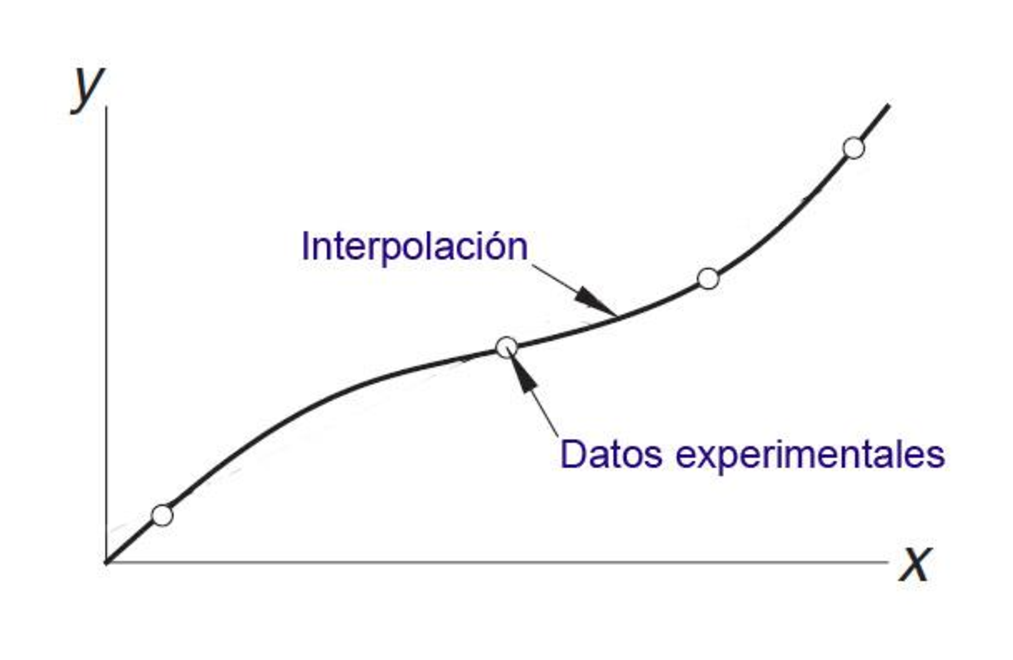
\includegraphics[scale=0.5]{Imagenes/Interpol02.eps}
\end{figure}
\end{frame}
\begin{frame}
\frametitle{Diferencia entre ajuste curvas e interpolación}
Ajuste de la curva:
\begin{figure}
   \centering
   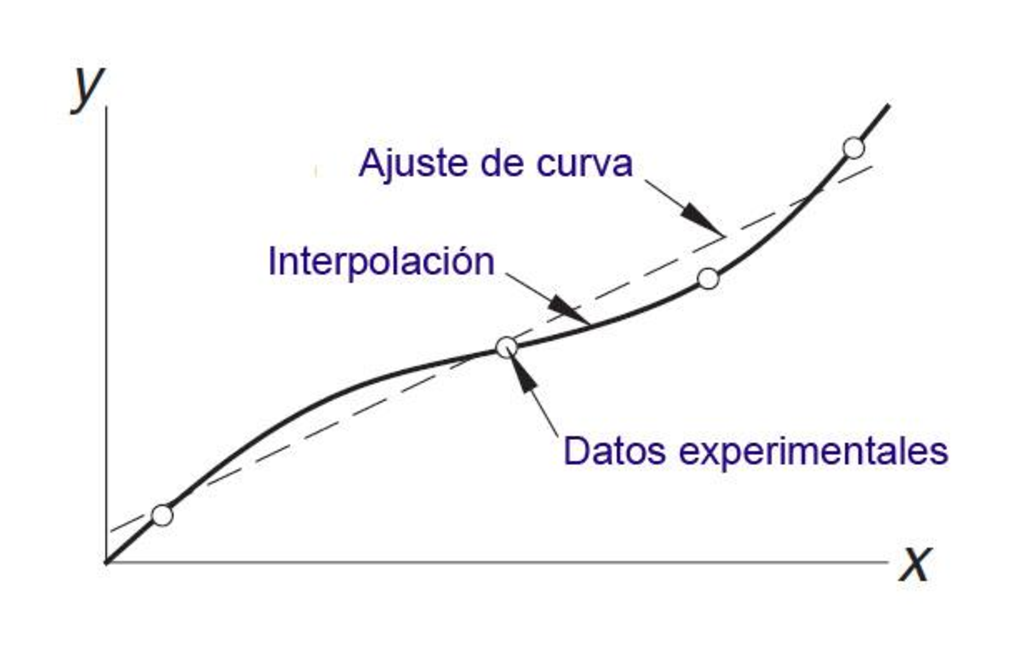
\includegraphics[scale=0.5]{Imagenes/Interpol03.eps}
\end{figure}
\end{frame}
\begin{frame}
\frametitle{Polinomio de interpolación}
Supongamos que lo que se quiere es buscar un polinomio de grado finito que aproxime una función dada.
\\
\bigskip
\pause
Lo que resulta intuitivo es buscar que dicho polinomio tenga el mismo valor de la función en un conjunto de puntos dado.
\end{frame}
\begin{frame}
\frametitle{Polinomio de interpolación}
Sabiendo que por $n$ puntos pasa un único polinomio de grado $n-1$, podríamos argumentar que la única manera de buscar una aproximación mejor del polinomio a la función es la de escoger de formas distintas los puntos por los cuales el polinomio ha de pasar.
\end{frame}
\begin{frame}
\frametitle{Polinomio de interpolación}
Dada una función $f(x)$ de la cual se conocen sus valores en un número finito de puntos $x_{0}, x_{1}, \ldots, x_{m}$, \pause se llama \textbf{\textcolor{red(ncs)}{interpolación polinómica}} al proceso de hallar un polinomio $p_{m}(x)$ de grado menor o igual a $m$, cumpliendo $p_{m}(x_{k}) = f(x_{k})$ parar cada $k = 1, 2, \ldots, m$.
\end{frame}
\begin{frame}
\frametitle{Polinomio de interpolación}
Los coeficientes $a_{0}, a_{1}, a_{2}, \ldots, a_{n}$, de dicho polinomio se obtienen imponiendo al polinomio de pasar por los puntos experimentales.
\end{frame}
\begin{frame}
\frametitle{Sistema matricial}
\begin{align*}
\mqty[
x_{0}^{n} & x_{0}^{n-1} & x_{0}^{n-2} & \ldots & x_{0} & 1 \\
x_{1}^{n} & x_{1}^{n-1} & x_{1}^{n-2} & \ldots & x_{1} & 1 \\
\vdots & \vdots & \vdots & & \vdots & \vdots \\
x_{n}^{n} & x_{n}^{n-1} & x_{n}^{n-2} & \ldots & x_{n} & 1 
]
\mqty[
a_{n} \\ a_{n-1} \\ \vdots \\ a_{0}
]
=
\mqty[
y_{0} \\ y_{1} \\ \vdots \\ y_{n}
]
\end{align*}
\end{frame}
\begin{frame}
\frametitle{Sistema matricial}
Este sistema es compatible y a la matriz asociada se le suele denominar \textocolor{richblack}{matriz de Vandermonde}.
\end{frame}
\begin{frame}
\frametitle{Complejidad computacional}
La complejidad computacional para invertir la matriz es de $\order{n^{3}}$.
\\
\bigskip
\pause
Por esta razón, han sido construidos diferentes algoritmos que aprovechan la particular estructura de este sistema que reducen la complejidad a $\order{n^{2}}$, \pause como el \textocolor{cadmiumgreen}{método de Lagrange} \pause o el \textocolor{blue(ryb)}{método de las diferencias divididas de Newton}.
\end{frame}

\section{Interpolación de Lagrange}
\frame[allowframebreaks]{\frametitle{Temas a revisar} \tableofcontents[currentsection, hideothersubsections]}
\subsection{El método de interpolación}

\begin{frame}
\frametitle{El método de Lagrange}
El polinomio interpolador de grado $n$ de Lagrange es un polinomio de la forma:
\pause
\begin{align*}
p_{n} (x) = \nsum_{j=0}^{k} f_{j} (x) \, l_{j} (x) \hspace{1.5cm} n \leq m
\end{align*}
\end{frame}
\begin{frame}
\frametitle{Polinomios de Lagrange}
Donde los $l_{j}(x)$ son los llamados \textocolor{burgundy}{polinomios de Lagrange}, que se calculan como:
\pause
\fontsize{12}{12}\selectfont
\begin{eqnarray*}
\begin{aligned}
&l_{j}(x) = \prod_{j \neq i} \dfrac{x - x_{i}}{x_{j} - x_{i}} = \\[0.5em] \pause
&= \dfrac{(x {-} x_{0})(x {-} x_{i}) \ldots(x {-} x_{j-1})(x {-} x_{j+1}) \ldots (x {-} x_{n})}{(x_{j} {-} x_{0})(x_{j} {-} x_{1}) \ldots(x_{j} {-} x_{j-1})(x_{j} {-} x_{j+1}) \ldots (x_{j} {-} x_{n})}
\end{aligned}
\end{eqnarray*}
\end{frame}
\begin{frame}
\frametitle{Ejemplo}
Se quiere hallar el valor de la función:
\pause
\begin{align*}
f (x) = e^{x+1}
\end{align*}
Utilizando un polinomio de interpolación de Lagrange de grado $2$ que pase por los puntos:
\pause
\fontsize{12}{12}\selectfont
\begin{table}
\centering
\begin{tabular}{c | c}
$x$ & $f(x)$ \\ \hline
$0$ & $f(0)$ \\
$0.5$ & $f(0.5)$ \\
$1$ & $f(1)$ \\
\end{tabular}
\end{table}
\end{frame}
\begin{frame}
\frametitle{Gráfica de los puntos}
Al graficar los puntos tendremos lo siguiente:
\begin{figure}
   \centering  
   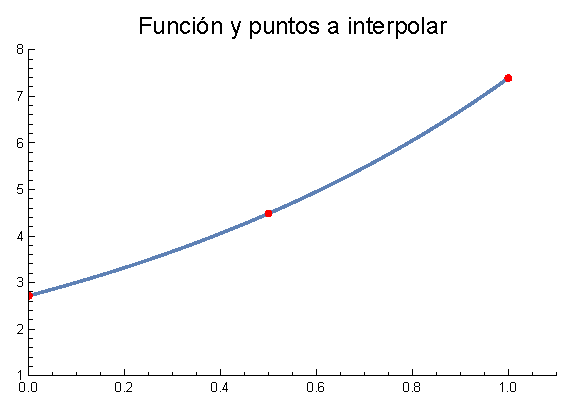
\includegraphics[scale=0.95]{Imagenes/Plot_Chebyshev_Ejercicio_Interp_01.eps}
\end{figure}
\end{frame}
\begin{frame}
\frametitle{Obteniendo los polinomios}
Usamos el método directo para calcular el polinomio de interpolación.
\end{frame}
\begin{frame}
\frametitle{Obteniendo los polinomios}
Con las condiciones dadas, los polinomios de Lagrange son:
\pause
\begin{eqnarray*}
\begin{aligned}
l_{0} (x) &= \dfrac{(x - 0.5)(x - 1)}{0.5} = \pause 2 \, x^{2} - 3 \, x + 1 \\[0.5em] \pause 
l_{1} (x) &= \dfrac{x (x - 1)}{-0.25} = \pause - 4 \, x^{2} + 4 \, x \\[0.5em] \pause
l_{2} (x) &= \dfrac{x (x - 0.5)}{0.5} = \pause 2 \, x^{2} - x
\end{aligned}
\end{eqnarray*}
\end{frame}
\begin{frame}
\frametitle{Polinomio de interpolación}
El polinomio de interpolación de Lagrange de grado $2$ es:
\pause
\begin{eqnarray*}
\begin{aligned}
p_{2} (x) &= \nsum_{j=0}^{2} f_{j}(x) \, l_{j}(x) = \\[0.5em] \pause
&= (2 \, e - 4 \, e^{3/2} + 2 \, e^{2}) \, x^{2} + \\[0.5em]
&+ (-3 \, e \, + 4 \, e^{3/2} + 2 \, e^{2}) \, x + e
\end{aligned}
\end{eqnarray*}
\end{frame}
\begin{frame}
\frametitle{Comparando el resultado}
\begin{figure}
    \centering
    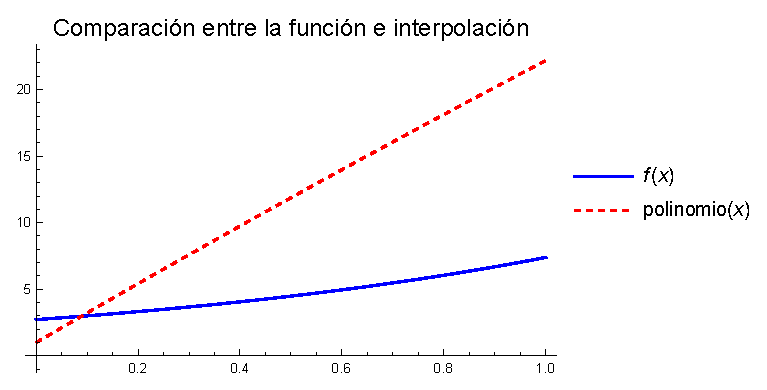
\includegraphics[scale=0.81]{Imagenes/Plot_Chebyshev_Ejercicio_Interp_02.eps}
\end{figure}
\end{frame}
\begin{frame}
\frametitle{Error de la aproximación}
Una pregunta que puede surgir al utilizar un polinomio de interpolación para aproximar una función es: \pause ¿qué tan bueno es el ajuste del polinomio a la función originaria?.
\end{frame}
\begin{frame}
\frametitle{Error de la aproximación}
Por esta razón consideramos el error de interpolación de un polinomio de grado $n$ que pase por los puntos de una función $f(x)$ en los puntos $x_{0}, \ldots, x_{n}$.
\end{frame}
\begin{frame}
\frametitle{Error de la aproximación}
Si $f(x)$ es una función determinada en $x_{0}, \ldots, x_{n}$ y es $n$ veces diferenciable, entonces el \textocolor{carmine}{error de interpolación} puede calcularse como valor absoluto de la diferencia entre la función y el polinomio.
\end{frame}
\begin{frame}
\frametitle{Error de la aproximación}
Construimos una función $\phi (x)$ por la cual se cumpla que:
\pause
\begin{align*}
&\phi(x) = f(x) {-} p_{n}(x) {-} a(x)(x {-} a_{0})(x {-} a_{1}) \ldots (x {-} a_{n}) \\[0.5em]
&\exists \, \bar{x} \in [-1, 1] \\[0.5em]
&a(\bar{x}) = \big[ f(x) {-} p_{n} \big] (x {-} a_{0})(x {-} a_{1}) \ldots (x {-} a_{n}) = 0
\end{align*}
\end{frame}
\begin{frame}
\frametitle{Error de interpolación}
Esta función se anula en $n + 2$ puntos. 
\\
\bigskip
\pause
Aplicando el \textocolor{crimsonglory}{teorema de Rolle} se tiene que una función que toma el mismo valor $n + 2$ veces tiene $n + 1$ puntos que anulan la derivada.
\end{frame}
\begin{frame}
\frametitle{Error de interpolación}
A la vez, la derivada de esta función es tal que, teniendo $n + 1$ puntos con el mismo valor tendrá $n$ puntos que anulan su derivada. 
\end{frame}
\begin{frame}
\frametitle{Error de interpolación}
Por lo tanto, derivando sucesivamente $n + 1$ veces, tenemos que existirá un único punto $\zeta$ que anule la derivada $n+1$-ésima, es decir:
\pause
\begin{align*}
\phi^{n+1} \, (\zeta) = 0
\end{align*}
\end{frame}
\begin{frame}
\frametitle{Error de interpolación}
Así podemos asegurar que $\phi^{n+1}$ tiene al menos una raíz, \pause con lo cual resulta evidente que, siendo $p_{n}(x)$ un polinomio de grado mayor que $n - 1$, $\phi^{n+1} \, (\zeta)$ resultará la siguiente:
\pause
\begin{align*}
\phi^{n+1} \, (x) = f^{(n+1)} \, (\bar{x}) - a (\bar{x}) (n + 1)!
\end{align*}
\end{frame}
\begin{frame}
\frametitle{Error de interpolación}
Por consiguiente, al haber dejado que en $\phi^{n+1} \, (\bar{x}) = 0$, se tiene que:
\pause
\begin{align*}
a (\bar{x}) = \dfrac{f^{(n+1)} \, (\bar{x})}{(n + 1)!}
\end{align*}
\end{frame}
\begin{frame}
\frametitle{Error de interpolación}
En el caso de que $f(x)$ sea $n$ veces diferenciable en el dominio $[-1, 1]$, el error de interpolación podrá definirse como:
\pause
\begin{align*}
f(x) - p_{n}(x) = \dfrac{f^{(n+1)}(\xi)}{(n + 1)!} \, \prod_{i} (x - x_{i})
\end{align*}
\pause
Donde $\xi$ es un punto que pertenece a $[-1, 1]$, por lo cual $\phi^{(n+1)}(\zeta) = 0$.
\end{frame}
\begin{frame}
\frametitle{Maximizando la expresión}
Dejamos los valores absolutos en la expresión del error de interpolación y maximizando ambos lados de la desigualdad a lo largo del intervalo $[-1, 1]$ obtenemos la cota para dicho error:
\pause
\begin{eqnarray*}
\begin{aligned}
&\max_{\abs{x} < 1} \abs{f(x) - p_{n}(x)} = \pause \abs{\dfrac{f^{(n+1)}(\xi)}{(n + 1)!} \, \prod_{i} (x - x_{i})} \leq \\[0.5em] \pause
&\leq \dfrac{\displaystyle \max_{\abs{x} < 1} \abs{f^{(n+1)}(\xi)}}{(n+1)!} \, \max_{\abs{x} < 1} \prod_{i} (x - x_{i})
\end{aligned}
\end{eqnarray*}
\end{frame}
\begin{frame}
\frametitle{Resultado del error}
Dada la unicidad del polinomio de interpolación, las únicas dos cosas que podemos mover a la hora de reducir el error de interpolación son:
\setbeamercolor{item projected}{bg=yellow,fg=black}
\setbeamertemplate{enumerate items}{%
\usebeamercolor[bg]{item projected}%
\raisebox{1.5pt}{\colorbox{bg}{\color{fg}\footnotesize\insertenumlabel}}%
}
\begin{enumerate}[<+->]
\item El grado del polinomio (por consiguiente, el número de puntos)
\item La localización de dichos puntos.
\end{enumerate}
\end{frame}
\begin{frame}
\frametitle{Resultado del error}
Se podría creer que al aumentar el grado del polinomio el error de interpolación se reduzca. 
\\
\bigskip
\pause
En realidad, pese al ser un resultado antiintuitivo, Carle David Tolmé Runge observó que el error de interpolación en un intervalo dado, tiende a infinito cuando el grado del polinomio de interpolación tiende a infinito.
\end{frame}
\begin{frame}
\frametitle{Resultado del error}
Es decir:
\pause
\begin{align*}
\lim_{n \to \infty} \big( \max_{\abs{x} < 1} \abs{f(x) - p_{n}(x)} \big) = \infty
\end{align*}
\end{frame}
\begin{frame}
\frametitle{Error mínimo}
El método que veremos nos permite proporcionar los puntos por los cuales hacer pasar el polinomio de interpolación de forma tal que la distancia máxima entre el polinomio interpolado y la función originaria sea mínima.
\end{frame}
\begin{frame}
\frametitle{Error mínimo}
La oscilación observada por Runge se puede minimizar usando nodos de Chebyshev en lugar de nodos equidistantes.
\\
\bigskip
\pause
En este caso se garantiza que el error máximo disminuye al crecer el orden polinómico.
\end{frame}

\section{Polinomios de Chebyshev}
\frame[allowframebreaks]{\frametitle{Temas a revisar} \tableofcontents[currentsection, hideothersubsections]}
\subsection{Usando las raíces}

\begin{frame}
\frametitle{Raíces de los polinomios}
Esta es una propiedad que hace particularmente interesante el utilizar las raíces de los polinomios de Chebyshev como puntos por donde interpolar el polinomio.
\end{frame}
\begin{frame}
\frametitle{Minimizando el error}
Para minimizar el último factor de la cota del error, Pafnuty Lvovich Chebyshev demostró que los puntos $x_{0}, \ldots, x_{n}$ por los cuales hacer pasar el polinomio, han de ser escogidos de forma que:
\pause
\begin{align*}
\max_{\abs{x}<1} \prod_{i} (x - x_{i}) = \dfrac{1}{2^{n}} \, T_{n+1} (x)
\end{align*}
donde $T_{n+1}(x)$ es el polinomio de Chebyshev de primera clase de orden $n + 1$.
\end{frame}
\begin{frame}
\frametitle{Elección de los puntos}
Entre todas las elecciones de los puntos $x_{0}, \ldots, x_{n}$, elegirlos de forma que la siguiente expresión se respete:
\pause
\begin{align*}
\phi^{n+1} \, (x) = f^{(n+1)} \, (\bar{x}) - a (\bar{x}) (n + 1)!
\end{align*}
\end{frame}
\begin{frame}
\frametitle{Elección de los puntos}
Se garantiza que el polinomio así obtenido es el polinomio único que tenga la propiedad:
\pause
\begin{eqnarray*}
\begin{aligned}
\max_{\abs{x}<1} T_{n} (x) &\leq \max_{\abs{x}<1} \prod (x - x_{i}) \\[0.5em] \pause
\max_{\abs{x}<1} T_{n} (x) &= \dfrac{1}{2^{n}} \\[0.5em]
\dfrac{1}{2^{n}} &\leq \max_{\abs{x}<1} T_{n} (x)
\end{aligned}
\end{eqnarray*}
\end{frame}
\begin{frame}
\frametitle{Error de interpolación}
Se puede demostrar que el valor absoluto de la diferencia entre la función y el polinomio interpolado por las raíces del polinomio de Chebyshev resulta acotado de la siguiente forma:
\pause
\begin{align*}
\abs{f(x) - p_{n-1}} \leq \dfrac{1}{2^{n-1} \, n!} \, \max_{\xi \in [-1, 1]}  \, \abs{f^{n} \, (\xi)}
\end{align*}
\end{frame}

\section{Las raíces de Chebyshev}
\frame[allowframebreaks]{\frametitle{Temas a revisar} \tableofcontents[currentsection, hideothersubsections]}
\subsection{Interpretación geométrica}

\begin{frame}
\frametitle{Raíces del polinomio Chebyshev}
Una interpretación geométrica de las raíces de Chebyshev es aquella según la cual estos se colocan en un segmento de longitud igual al diámetro de un círculo, cuya circunferencia repartimos en $n$ partes iguales.
\end{frame}
\begin{frame}
\frametitle{Raíces del polinomio Chebyshev}
Proyectando a lo largo del dicho segmento el punto medio de cada partición de la semicirconferencia obtenemos puntos que coinciden con las raíces del polinomio de Chebyshev.
\begin{figure}
    \centering
    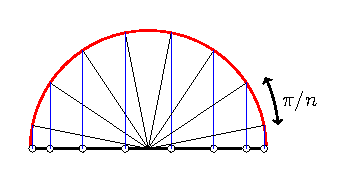
\includegraphics[scale=1]{Imagenes/Nodos_Chebychev_01.eps}
\end{figure}
\end{frame}
\begin{frame}
\frametitle{Minimizando el efecto Runge}
La razón por la cual la aproximación de una función $f (x)$ por un polinomio que interpole puntos escogidos de esta forma minimiza el efecto Runge, \pause es que la densidad de puntos resulta creciente desde el centro hasta las extremidades.
\end{frame}
\begin{frame}
\frametitle{Minimizando el efecto Runge}
Para calcular dichas raíces utiliza la identidad trigonométrica del polinomio de Chebyshev:
\pause
\begin{align*}
T_{n}(x) = \cos (n \, \arccos x) = \cosh (n \, \mbox{arccosh} \, x)
\end{align*}
\pause
Este coseno se anula cuando la expresión al interior es un múltiplo de $2 \, \pi$.
\end{frame}
\begin{frame}
\frametitle{Raíces polinomio Chebyshev}
Por lo tanto las raíces del polinomio de Chebyshev en $[-1, 1]$ son:
\pause
\begin{align*}
x_{i} = \cos \left( \dfrac{2 \, i - 1}{2 \, n} \, \pi \right) \hspace{1cm} i = 1, 2, \ldots, n
\end{align*}
\end{frame}
\begin{frame}
\frametitle{Raíces polinomio Chebyshev}
En el caso de que se quisiera definir el polinomio de Chebyshev en un intervalo cualquiera $[a, b]$, las raíces se trasforman como:
\pause
\begin{align*}
x_{i} = \dfrac{a + b}{2} &+ \dfrac{b - a}{2} \, \cos \left( \dfrac{2 \, i - 1}{2 \, n} \, \pi \right) \\[0.5em] 
i =& 0, 1, \ldots, n
\end{align*}
\end{frame}
\begin{frame}
\frametitle{Obteniendo coeficientes}
La utilización de los nodos de Chebyshev nos permite también utilizar un método recursivo para la obtención de los coeficientes:
\pause
\begin{align*}
f (x) \simeq \nsum_{j=0}^{n} c_{j} \, T_{j}(x)
\end{align*}
donde los coeficientes $c_{j}$ son:
\end{frame}
\begin{frame}
\frametitle{Obteniendo coeficientes}
Los coeficientes $c_{j}$ son:
\pause
\begin{align*}
c_{0} &= \dfrac{1}{n + 1} \, \nsum_{j=0}^{n} f(x_{k}) \, T_{0}(x_{k}) = \dfrac{1}{n + 1} \, \nsum_{j=0}^{n} f(x_{k}) \\[1em]
c_{j} &= \dfrac{1}{n + 1} \, \nsum_{j=0}^{n} f(x_{k}) \, T_{j}(x_{k})
\end{align*}
\end{frame}
\begin{frame}
\frametitle{Usando los coeficientes}
Esta fórmula permita calcular los coeficientes del polinomio de interpolación con un costo computacional del orden de $\order{n^{2}}$ operaciones.
\end{frame}

\section{Ejercicio}
\frame[allowframebreaks]{\frametitle{Temas a revisar} \tableofcontents[currentsection, hideothersubsections]}
\subsection{Ajuste polinomial}

\begin{frame}
\frametitle{Enunciado}
Consideramos la función:
\begin{align*}
f (x) = \dfrac{800 \, x}{54 \, x^{4} + x^{2} + 3}
\end{align*}
para interpolar dos polinomios de igual grado a los puntos de dicha función, en el intervalo $[-1, 1]$.
\end{frame}
\begin{frame}
\frametitle{Gráfica de la función}
La función a interpolar es la siguiente:
\begin{figure}
    \centering
    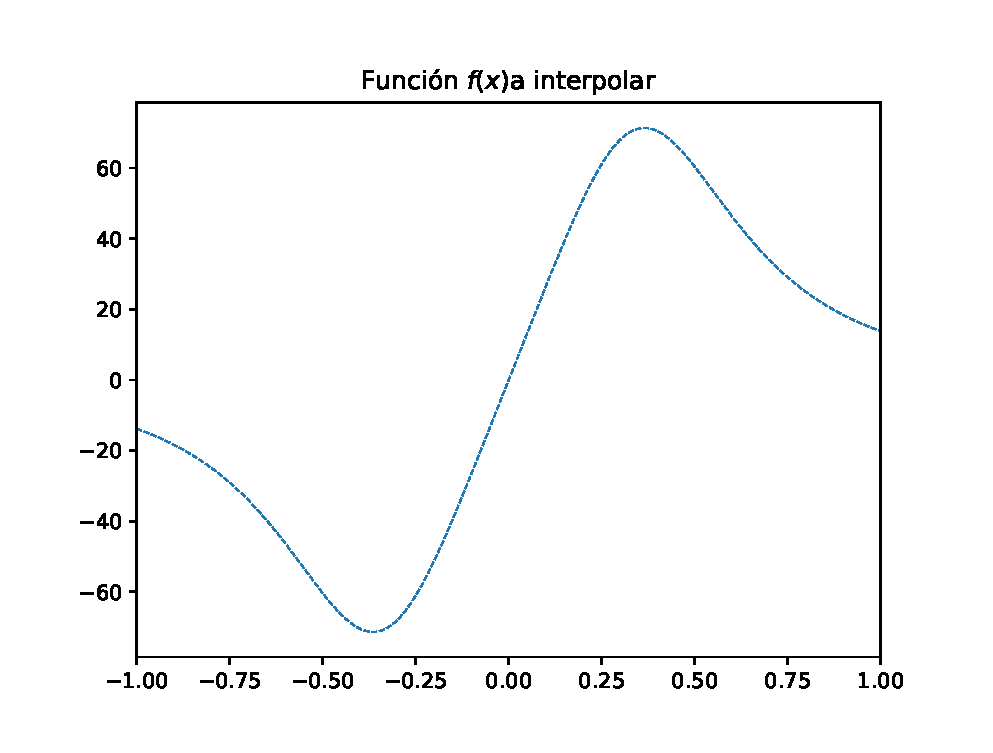
\includegraphics[scale=0.5]{Imagenes/Plot_Ejercicio_Chebychev_01.eps}
\end{figure}
\end{frame}
\begin{frame}
\frametitle{Estrategia} 
El primer polinomio lo interpolamos con puntos equidistantes y el segundo con las raíces del polinomio de Chebyshev.
\\
\bigskip
\pause
Utilizamos dos medidas de distancia para evaluar la bondad de la aproximación:
\end{frame}
\begin{frame}
\frametitle{Evaluando la aproximación}
El error debido a la diferencia del área al cuadrado entre la función y el polinomio de interpolación:
\pause
\begin{align*}
d_{1} (f, p) = \scaleint{6ex}_{\bs a}^{b} \big[ f(x) - p(x) \big]^{2} \dd{x}
\end{align*}
\end{frame}
\begin{frame}
\frametitle{Segundad medida de aproximación}
La segunda medida para medir la bondad de la aproximación es la distancia máxima entre los puntos entre la función y el polinomio de interpolación:
\pause
\begin{align*}
d_{2} (f, p) = \max_{x} \abs{f(x) - p(x)}
\end{align*}
\end{frame}

\section{Implementación con python}
\frame[allowframebreaks]{\frametitle{Temas a revisar} \tableofcontents[currentsection, hideothersubsections]}
\subsection{Usando las librerías de python}

\begin{frame}
\frametitle{Usando python}
Con la finalidad de ocupar un lenguaje más versátil para resolver el ejercicio, usamos \textcolor{blue}{\texttt{python}} y las librerías con las cuales podremos obtener los valores de $d_{1}$ y $d_{2}$.
\end{frame}
\begin{frame}
\frametitle{Usando python}    
También con \textcolor{blue}{\texttt{python}} se elaboraron las gráficas de los procesos de aproximación con los puntos equidistantes y con los puntos de las raíces de los polinomios de Chebyshev.
\end{frame}
\begin{frame}
\frametitle{Librerías}
Se han ocupado las siguientes librerías:
\setbeamercolor{item projected}{bg=yellow,fg=black}
\setbeamertemplate{enumerate items}{%
\usebeamercolor[bg]{item projected}%
\raisebox{1.5pt}{\colorbox{bg}{\color{fg}\footnotesize\insertenumlabel}}%
}
\begin{enumerate}[<+->]
\item \texttt{numpy.polyfit} 
\item \texttt{numpy.poly1d}.
\item \texttt{scipy.integrate.quad}
\item \texttt{scipy.special.roots\_chebyt}
\item \texttt{matplotlib.pyplot}
\end{enumerate}
\end{frame}

\subsection{Obteniendo las aproximaciones}

\begin{frame}
\frametitle{Resolviendo el problema}
Se calculan $d_{1}$, $d_{2}$, así como las gráficas del ajuste polinomial con puntos equidistantes y con las raíces del polinomio de Chebyshev para el conjunto de puntos:
\pause
\begin{align*}
n = 3, 5, 8, 10, 12, 14, 16
\end{align*}
que se presentan a continuación:
\end{frame}
\begin{frame}
\frametitle{Con $n = 3$}
    \centering
    \includegraphics<1>[scale=0.6]{Imagenes/Interpolacion_Chebychev_03_Polinomio.eps}% 
    \includegraphics<2>[scale=0.6]{Imagenes/Interpolacion_Chebychev_03_Raices.eps}
\end{frame}
\begin{frame}
\frametitle{Con $n = 5$}
    \centering
    \includegraphics<1>[scale=0.6]{Imagenes/Interpolacion_Chebychev_05_Polinomio.eps}% 
    \includegraphics<2>[scale=0.6]{Imagenes/Interpolacion_Chebychev_05_Raices.eps}
\end{frame}
\begin{frame}
\frametitle{Con $n = 8$}
    \centering
    \includegraphics<1>[scale=0.6]{Imagenes/Interpolacion_Chebychev_08_Polinomio.eps}% 
    \includegraphics<2>[scale=0.6]{Imagenes/Interpolacion_Chebychev_08_Raices.eps}
\end{frame}
\begin{frame}
\frametitle{Con $n = 10$}
    \centering
    \includegraphics<1>[scale=0.6]{Imagenes/Interpolacion_Chebychev_10_Polinomio.eps}% 
    \includegraphics<2>[scale=0.6]{Imagenes/Interpolacion_Chebychev_10_Raices.eps}
\end{frame}
\begin{frame}
\frametitle{Con $n = 12$}
    \centering
    \includegraphics<1>[scale=0.6]{Imagenes/Interpolacion_Chebychev_12_Polinomio.eps}% 
    \includegraphics<2>[scale=0.6]{Imagenes/Interpolacion_Chebychev_12_Raices.eps}
\end{frame}
\begin{frame}
\frametitle{Con $n = 14$}
    \centering
    \includegraphics<1>[scale=0.6]{Imagenes/Interpolacion_Chebychev_14_Polinomio.eps}% 
    \includegraphics<2>[scale=0.6]{Imagenes/Interpolacion_Chebychev_14_Raices.eps}
\end{frame}
\begin{frame}
\frametitle{Con $n = 16$}
    \centering
    \includegraphics<1>[scale=0.6]{Imagenes/Interpolacion_Chebychev_16_Polinomio.eps}% 
    \includegraphics<2>[scale=0.6]{Imagenes/Interpolacion_Chebychev_16_Raices.eps}
\end{frame}
\begin{frame}
\frametitle{Resumen}
\begin{table}
    \fontsize{12}{12}\selectfont
\begin{tabular}{| c | c | c |} \hline
puntos & $d_{1}$ & $d_{2}$ \\\hline
\multirow{2}{*}{$3$} & $3281.06$ & $66.33$ \\
 & $2799.63$ & $62.98$ \\ \hline
 \multirow{2}{*}{$5$} & $709.14$ & $28.11$ \\
 & $714.92$ & $34.66$ \\ \hline 
 \multirow{2}{*}{$8$} & $19.85$ & $5.68$ \\
 & $6.82$ & $4.12$ \\ \hline
\end{tabular}
\end{table}
\end{frame}
\begin{frame}
\frametitle{Resumen}
\begin{minipage}[t]{0.4\textwidth}
\begin{table}
\renewcommand{\arraystretch}{0.99}
\fontsize{12}{12}\selectfont
\begin{tabular}{| c | c | c |} \hline
puntos & $d_{1}$ & $d_{2}$ \\\hline
\multirow{2}{*}{$10$} & $317.75$ & $37.95$ \\
    & $6.99$ & $3.82$ \\ \hline
    \multirow{2}{*}{$12$} & $478.56$ & $52.64$ \\
    & $3.0$ & $2.31$ \\ \hline 
    \multirow{2}{*}{$14$} & $164.88$ & $35.73$ \\
    & $0.6$ & $1.01$ \\ \hline
\end{tabular}
\end{table}
\end{minipage}
\hspace{0.6cm}
\begin{minipage}[t]{0.4\textwidth}
\begin{table}
\fontsize{12}{12}\selectfont
\begin{tabular}{| c | c | c |} \hline
puntos & $d_{1}$ & $d_{2}$ \\\hline
\multirow{2}{*}{$16$} & $44.12$ & $19.73$ \\
    & $0.05$ & $0.32$ \\ \hline
\end{tabular}
\end{table}
\end{minipage}
\end{frame}
\begin{frame}
\frametitle{Conclusiones}
Lo que encontramos claramente es que el método con las raíces del polinomio de Chebyshev resulta óptimo para la minimización de la mayor distancia existente entre la función que se desea aproximar $f (x)$ y el polinomio que se construye con las raíces de Chebyshev.
\end{frame}
\begin{frame}
\frametitle{Conclusiones}
Sin embargo, esto no garantiza de ninguna forma la minimización del otras distancias, como se observó en caso de la norma $d_{1}$.
\end{frame}
\begin{frame}
\frametitle{Conclusiones}
Un inconveniente considerable de dicho método es que si queremos añadir más puntos, se tendría que estimar de nuevo los coeficientes de los polinomios de Chebyshev.
\end{frame}
\begin{frame}
\frametitle{Conclusiones}
Con un algoritmo en \textcolor{blue}{\texttt{python}}, se simplifica esta tarea ya que el cálculo se realiza nuevamente al modificar el número de puntos $n$, las demás tareas ya quedan establecidas en funciones que se mandan llamar.
\end{frame}

\end{document}